\newpage
\section{Interpretability}
To answer the final research question; \textit{Do these data profiles provide more interpretability of error detection tools?}; the results from the experiments as described in \autoref{sec:interpretabilityoftools} will be showed in this section.

\subsection{Feature selection}
% Permutation importance feature selection
To improve machine learning models, dimensionality reduction can be a solution. Permutation importance was calculated for all the features of the dataset profiles for the best performing strategies, after all the estimators were trained. All the features that had a positive impact on the model prediction outcome were kept. 46 out of the original 72 features were kept. Now, using this hindsight information, the models were retrained with only those features. To compare the two sets of features used, the mean squared error (MSE) and median absolute error (MAE) are shown in \autoref{tab:improvements_feature_selection}. It shows that the improvements are negligible.

\begin{table}[h]
\centering
\begin{tabular}{l|ll|ll}
\textbf{Metric} & \textbf{MSE 1} & \textbf{MAE 1} & \textbf{MSE 2} & \textbf{MAE 2} \\ \hline
Precision       & 0.0543         & 0.0949         & 0.0532         & 0.0948         \\
Recall          & 0.1045         & 0.166          & 0.1048         & 0.1578         \\
Direct F1       & 0.0442         & 0.1006         & 0.0440         & 0.1007         \\
Combined F1     & 0.0452         & 0.0790         & 0.0455         & 0.0775        
\end{tabular}
\caption{Estimation score comparison (1 all features / 2 reduced number of features)}
\label{tab:improvements_feature_selection}
\end{table}


\subsection{Feature importance}
The feature importance will of the dataset profile features will be analyzed using SHAP values of the estimators produced in \autoref{sec:performanceprediction}

\subsubsection{General F1-score analysis}
For every best scoring strategy per tool, the feature importance analysis of the direct F1-estimator was done. The extensive results can be found in \autoref{app:feature_importances}. 
The key takeaways were that for every tool, an increase in $cells\_length\_variance$ and/or  $characters\_alphabet\_variance$ would have a negative impact on the performance (F1).
This can be contributed to the fact that whenever lengths of cells and the number of alphabetical characters, the data is less structured. Less structured data seems harder to detect errors in.

% ---------------------------------------------
% ---------------------------------------------
% ---------------------------------------------
% ---------------------------------------------
% ---------------------------------------------
% ---------------------------------------------

\subsubsection{ActiveClean}
\begin{figure}[H]
    \centering
    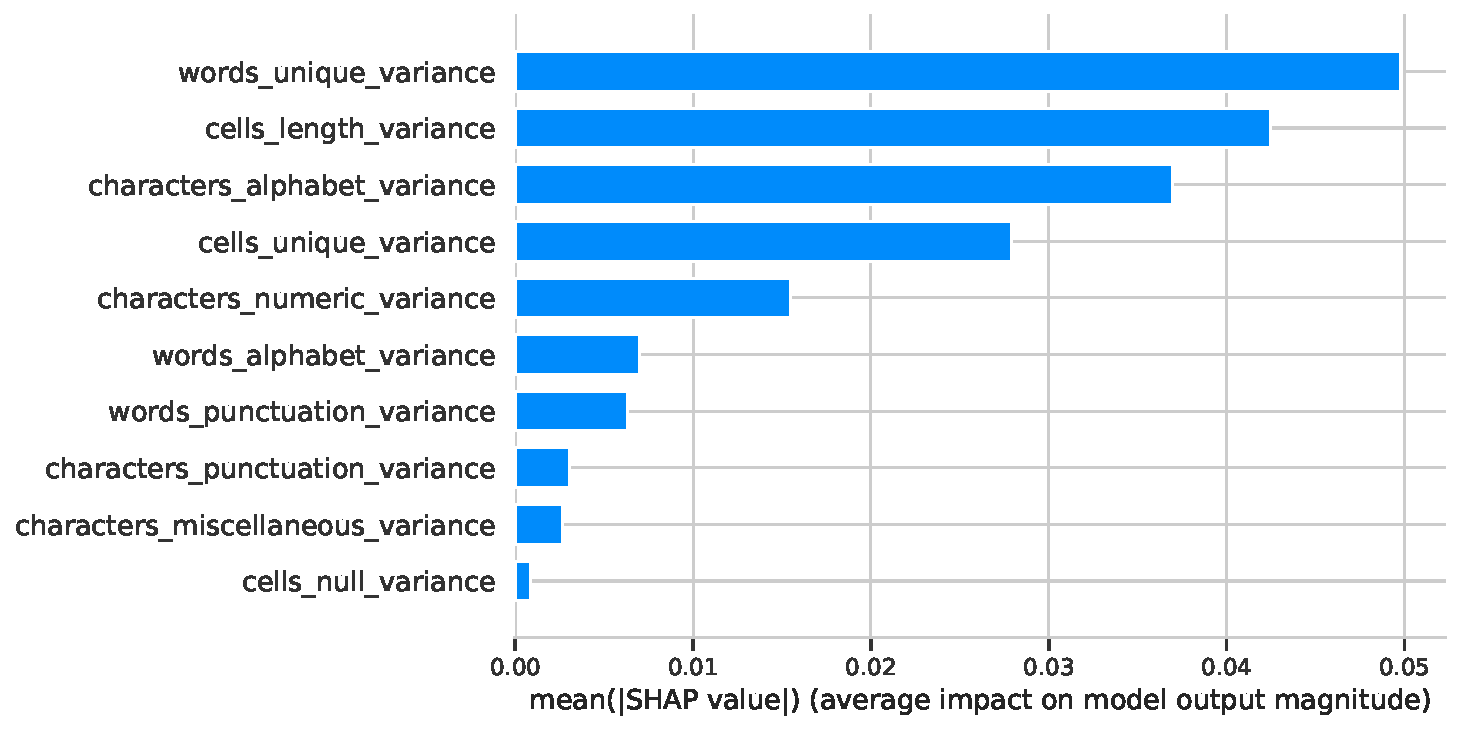
\includegraphics[width=0.9\textwidth]{thesis/Figures/RQ4/Shap_cell_prec_ActiveClean.pdf}
    \caption{ActiveClean - Top 10 Precision influential features according to SHAP values}
    \label{fig:feature_importance_prec_ActiveClean}
\end{figure}
\begin{figure}[H]
    \centering
    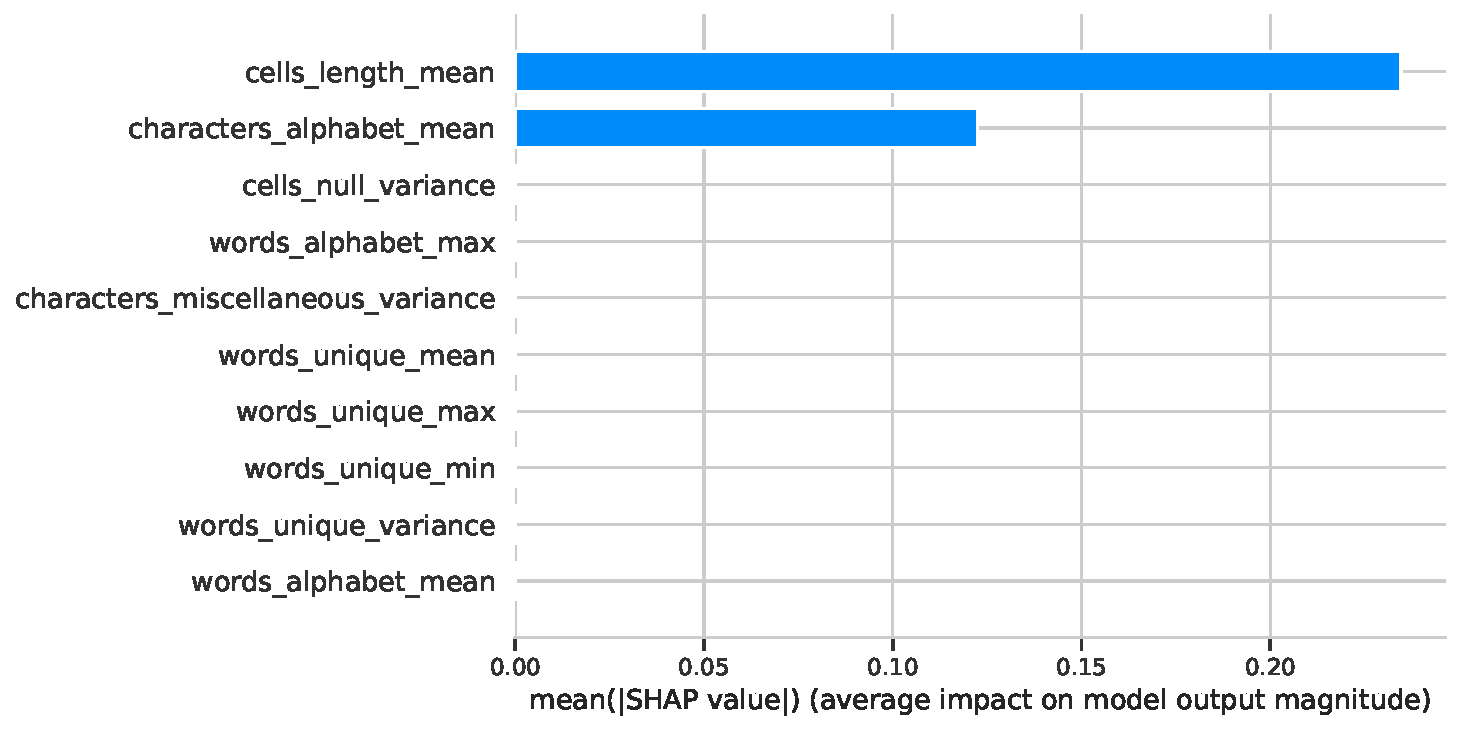
\includegraphics[width=0.9\textwidth]{thesis/Figures/RQ4/Shap_cell_rec_ActiveClean.pdf}
    \caption{ActiveClean - Top 10 Recall influential features according to SHAP values}
    \label{fig:feature_importance_rec_ActiveClean}
\end{figure}

\begin{table}[H]
	\centering
	\addtolength{\leftskip} {-2cm}
	\addtolength{\rightskip}{-2cm}
	\captionsetup[subtable]{position = below}
	\captionsetup[table]{position=top}
	\caption{Top feature influences - ActiveClean}
	\label{tab:feature_influences_ActiveClean}
		\begin{subtable}{0.5\linewidth}
		\centering
		\begin{tabular}{llr}
\toprule
 \# &                         Feature &         Influence \\
\midrule
 1 &         words\_unique\_variance &   0.39 $\nearrow$ \\
 2 &         cells\_length\_variance &  -0.42 $\searrow$ \\
 3 &  characters\_alphabet\_variance &  -0.39 $\searrow$ \\
\bottomrule
\end{tabular}
		\caption{Precision feature influences - ActiveClean}
		\label{tab:prec_feature_influences_ActiveClean}
	\end{subtable}
	\hspace*{4em}
	\begin{subtable}{0.5\linewidth}
		\centering
		\begin{tabular}{llr}
\toprule
 \# &                     Feature &         Influence \\
\midrule
 1 &         cells\_length\_mean &  -0.09 $\searrow$ \\
 2 &  characters\_alphabet\_mean &  -0.12 $\searrow$ \\
 3 &       cells\_null\_variance &                 0 \\
\bottomrule
\end{tabular}
		\caption{Recall feature influences - ActiveClean}
		\label{tab:rec_feature_influences_ActiveClean}
	\end{subtable}%
\end{table}

% ---------------------------------------------
% ---------------------------------------------
% ---------------------------------------------
% ---------------------------------------------
% ---------------------------------------------
% ---------------------------------------------


\subsubsection{dBoost}
\begin{figure}[H]
    \centering
    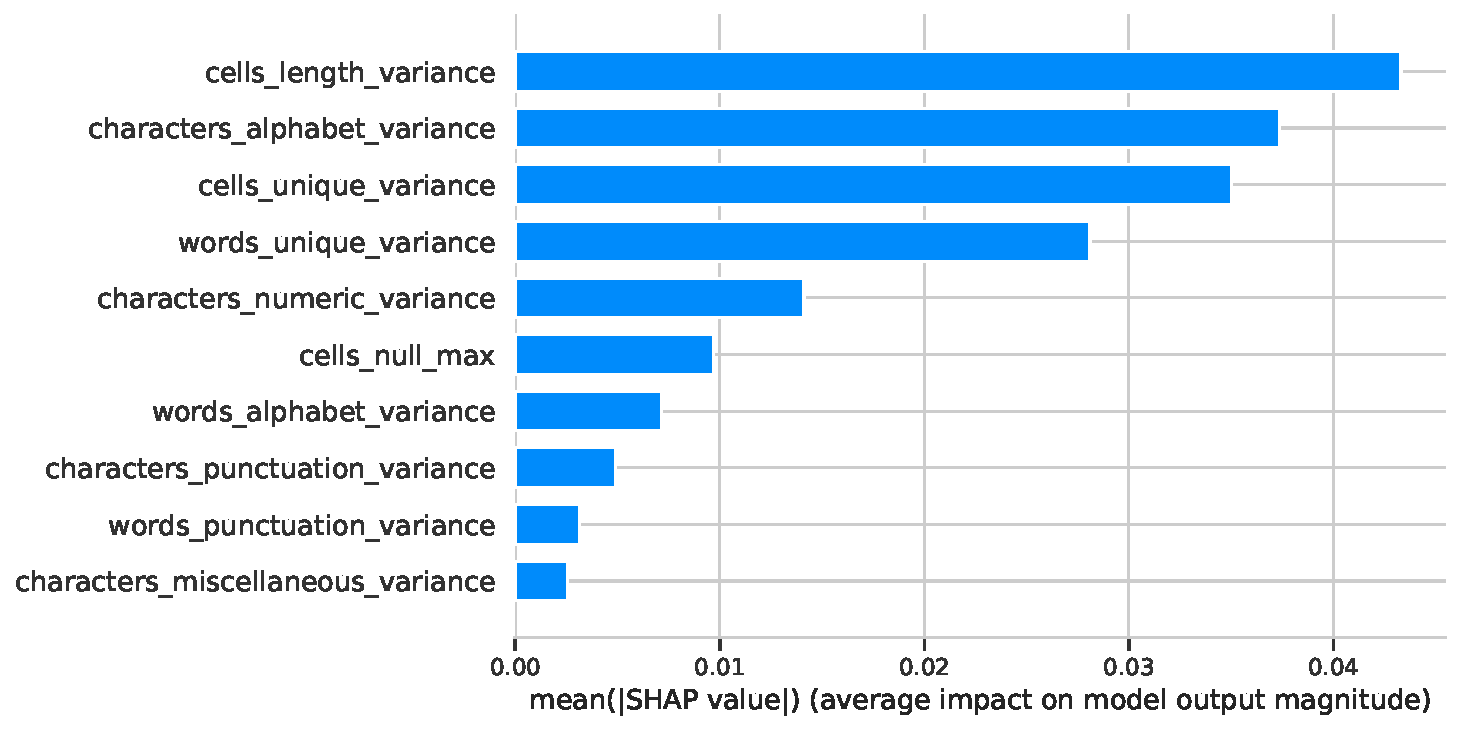
\includegraphics[width=0.9\textwidth]{thesis/Figures/RQ4/Shap_cell_prec_dBoost.pdf}
    \caption{dBoost - Top 10 Precision influential features according to SHAP values}
    \label{fig:feature_importance_prec_dBoost}
\end{figure}
\begin{figure}[H]
    \centering
    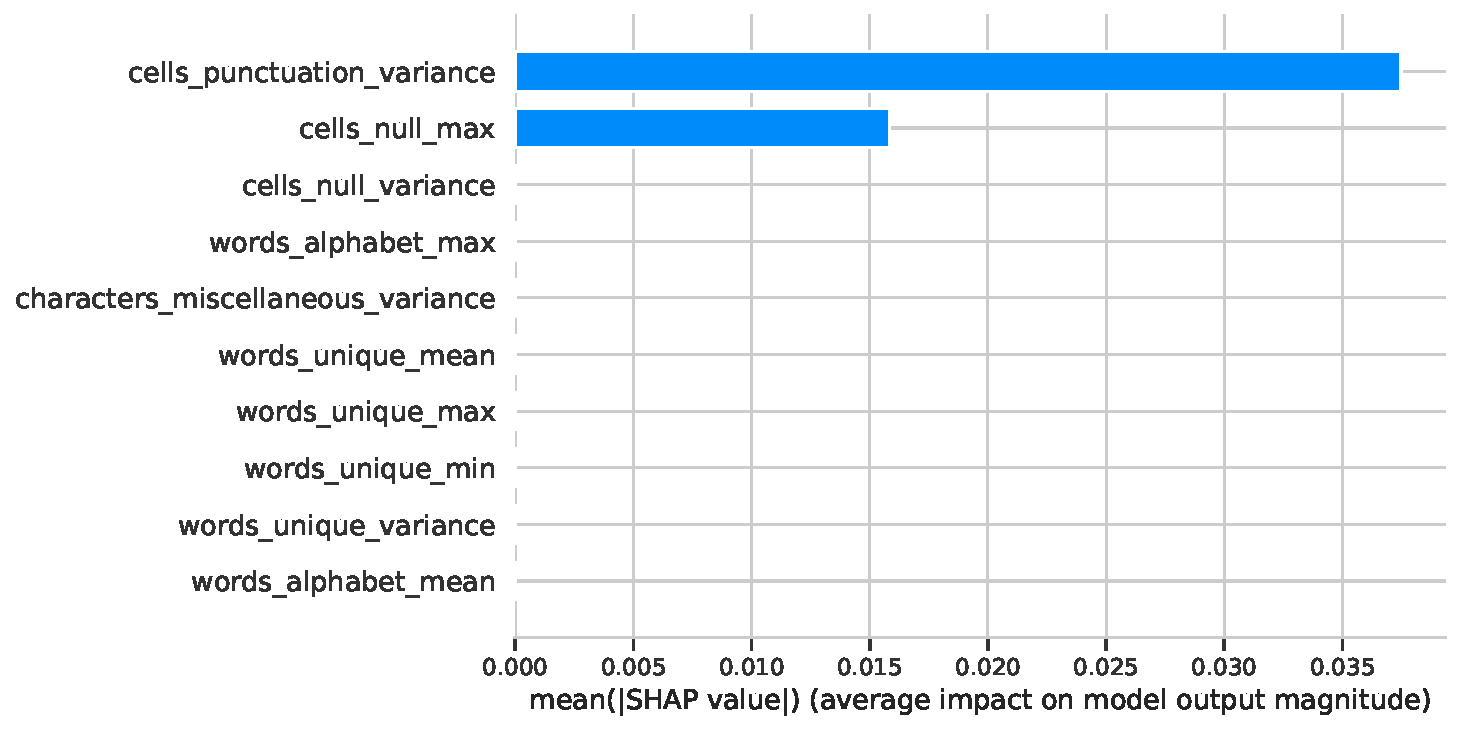
\includegraphics[width=0.9\textwidth]{thesis/Figures/RQ4/Shap_cell_rec_dBoost.pdf}
    \caption{dBoost - Top 10 Recall influential features according to SHAP values}
    \label{fig:feature_importance_rec_dBoost}
\end{figure}

\begin{table}[H]
	\centering
	\addtolength{\leftskip} {-2cm}
	\addtolength{\rightskip}{-2cm}
	\captionsetup[subtable]{position = below}
	\captionsetup[table]{position=top}
	\caption{Top feature influences - dBoost}
	\label{tab:feature_influences_dBoost}
		\begin{subtable}{0.5\linewidth}
		\centering
		\begin{tabular}{llr}
\toprule
 \# &                         Feature &         Influence \\
\midrule
 1 &         cells\_length\_variance &  -0.79 $\searrow$ \\
 2 &  characters\_alphabet\_variance &  -0.59 $\searrow$ \\
 3 &         cells\_unique\_variance &   0.72 $\nearrow$ \\
\bottomrule
\end{tabular}
		\caption{Precision feature influences - dBoost}
		\label{tab:prec_feature_influences_dBoost}
	\end{subtable}
	\hspace*{4em}
	\begin{subtable}{0.5\linewidth}
		\centering
		\begin{tabular}{llr}
\toprule
 \# &                       Feature &         Influence \\
\midrule
 1 &  cells\_punctuation\_variance &  -0.39 $\searrow$ \\
 2 &              cells\_null\_max &   0.29 $\nearrow$ \\
 3 &         cells\_null\_variance &                 0 \\
\bottomrule
\end{tabular}
		\caption{Recall feature influences - dBoost}
		\label{tab:rec_feature_influences_dBoost}
	\end{subtable}%
\end{table}

% ---------------------------------------------
% ---------------------------------------------
% ---------------------------------------------
% ---------------------------------------------
% ---------------------------------------------
% ---------------------------------------------

\subsubsection{FAHES}
\begin{figure}[H]
    \centering
    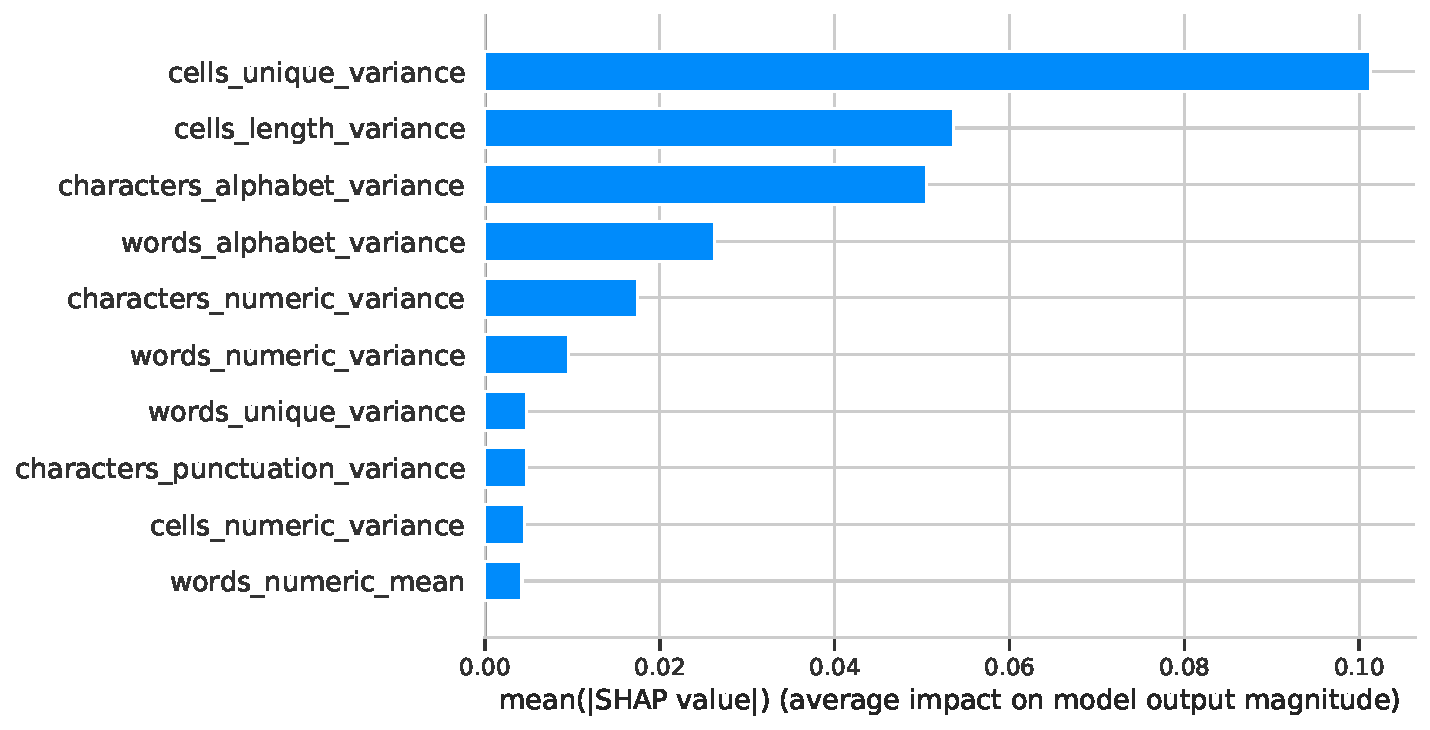
\includegraphics[width=0.9\textwidth]{thesis/Figures/RQ4/Shap_cell_prec_FAHES.pdf}
    \caption{FAHES - Top 10 Precision influential features according to SHAP values}
    \label{fig:feature_importance_prec_FAHES}
\end{figure}
\begin{figure}[H]
    \centering
    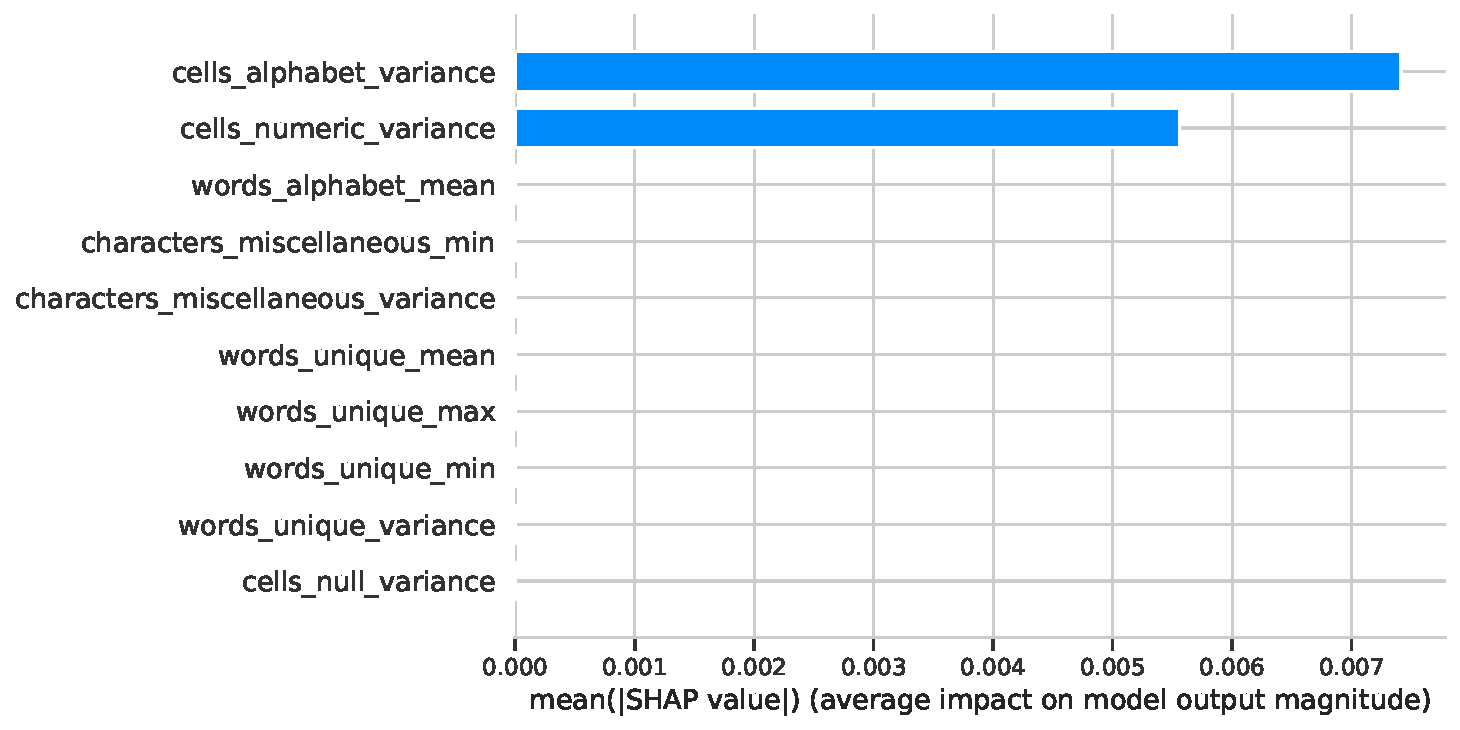
\includegraphics[width=0.9\textwidth]{thesis/Figures/RQ4/Shap_cell_rec_FAHES.pdf}
    \caption{FAHES - Top 10 Recall influential features according to SHAP values}
    \label{fig:feature_importance_rec_FAHES}
\end{figure}


\begin{table}[H]
	\centering
	\addtolength{\leftskip} {-2cm}
	\addtolength{\rightskip}{-2cm}
	\captionsetup[subtable]{position = below}
	\captionsetup[table]{position=top}
	\caption{Top feature influences - FAHES}
	\label{tab:feature_influences_FAHES}
		\begin{subtable}{0.5\linewidth}
		\centering
		\begin{tabular}{llr}
\toprule
 \# &                         Feature &         Influence \\
\midrule
 1 &         cells\_unique\_variance &   0.67 $\nearrow$ \\
 2 &         cells\_length\_variance &  -0.59 $\searrow$ \\
 3 &  characters\_alphabet\_variance &  -0.59 $\searrow$ \\
\bottomrule
\end{tabular}
		\caption{Precision feature influences - FAHES}
		\label{tab:prec_feature_influences_FAHES}
	\end{subtable}
	\hspace*{4em}
	\begin{subtable}{0.5\linewidth}
		\centering
		\begin{tabular}{llr}
\toprule
 \# &                    Feature &        Influence \\
\midrule
 1 &  cells\_alphabet\_variance &  0.66 $\nearrow$ \\
 2 &   cells\_numeric\_variance &  0.61 $\nearrow$ \\
 3 &      words\_alphabet\_mean &                0 \\
\bottomrule
\end{tabular}
		\caption{Recall feature influences - FAHES}
		\label{tab:rec_feature_influences_FAHES}
	\end{subtable}%
\end{table}

% ---------------------------------------------
% ---------------------------------------------
% ---------------------------------------------
% ---------------------------------------------
% ---------------------------------------------
% ---------------------------------------------


\subsubsection{Forbidden Itemsets}
\begin{figure}[H]
    \centering
    \includegraphics[width=0.9\textwidth]{thesis/Figures/RQ4/Shap_cell_prec_ForbiddenItemsets.pdf}
    \caption{Forbidden Itemsets - Top 10 Precision influential features according to SHAP values}
    \label{fig:feature_importance_prec_ForbiddenItemsets}
\end{figure}
\begin{figure}[H]
    \centering
    \includegraphics[width=0.9\textwidth]{thesis/Figures/RQ4/Shap_cell_rec_ForbiddenItemsets.pdf}
    \caption{Forbidden Itemsets - Top 10 Recall influential features according to SHAP values}
    \label{fig:feature_importance_rec_ForbiddenItemsets}
\end{figure}

\begin{table}[H]
	\centering
	\addtolength{\leftskip} {-2cm}
	\addtolength{\rightskip}{-2cm}
	\captionsetup[subtable]{position = below}
	\captionsetup[table]{position=top}
	\caption{Top feature influences - Forbidden Itemsets}
	\label{tab:feature_influences_ForbiddenItemsets}
		\begin{subtable}{0.5\linewidth}
		\centering
\begin{tabular}{llr}
\toprule
 \# &                  Feature &          Influence \\
\midrule
 1 &  cells\_length\_variance &    0.36 $\nearrow$ \\
 2 &  cells\_unique\_variance &  0.0 $\rightarrow$ \\
 3 &  words\_unique\_variance &   -0.18 $\searrow$ \\
\bottomrule
\end{tabular}
		\caption{Precision feature influences - Forbidden Itemsets}
		\label{tab:prec_feature_influences_ForbiddenItemsets}
	\end{subtable}
	\hspace*{4em}
	\begin{subtable}{0.5\linewidth}
		\centering
\begin{tabular}{llr}
\toprule
 \# &                  Feature &        Influence \\
\midrule
 1 &  words\_length\_variance &   0.3 $\nearrow$ \\
 2 &       words\_length\_min &  0.23 $\nearrow$ \\
 3 &     words\_alphabet\_min &                0 \\
\bottomrule
\end{tabular}
		\caption{Recall feature influences - Forbidden Itemsets}
		\label{tab:rec_feature_influences_ForbiddenItemsets}
	\end{subtable}%
\end{table}

% ---------------------------------------------
% ---------------------------------------------
% ---------------------------------------------
% ---------------------------------------------
% ---------------------------------------------
% ---------------------------------------------


\subsubsection{KATARA}
\begin{figure}[H]
    \centering
    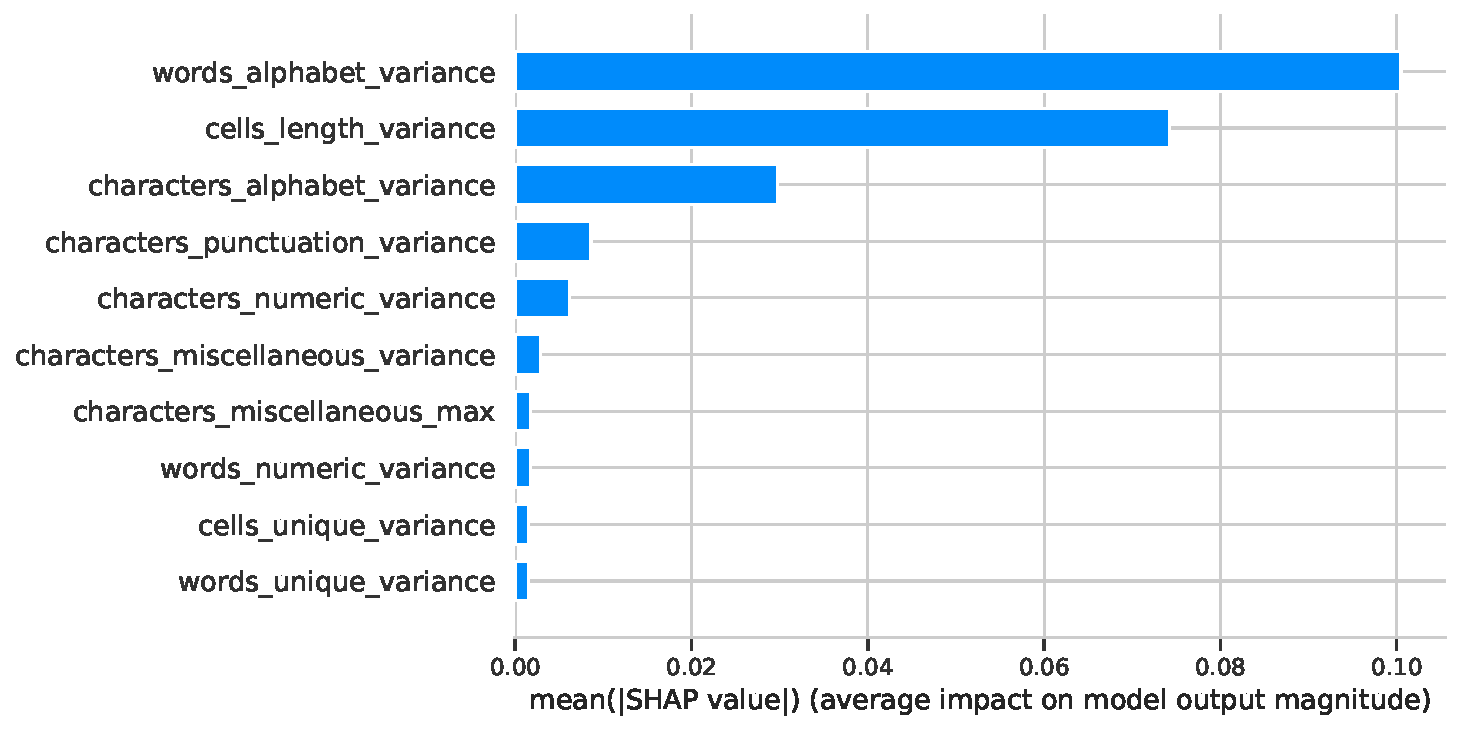
\includegraphics[width=0.9\textwidth]{thesis/Figures/RQ4/Shap_cell_prec_KATARA.pdf}
    \caption{KATARA - Top 10 Precision influential features according to SHAP values}
    \label{fig:feature_importance_prec_KATARA}
\end{figure}
\begin{figure}[H]
    \centering
    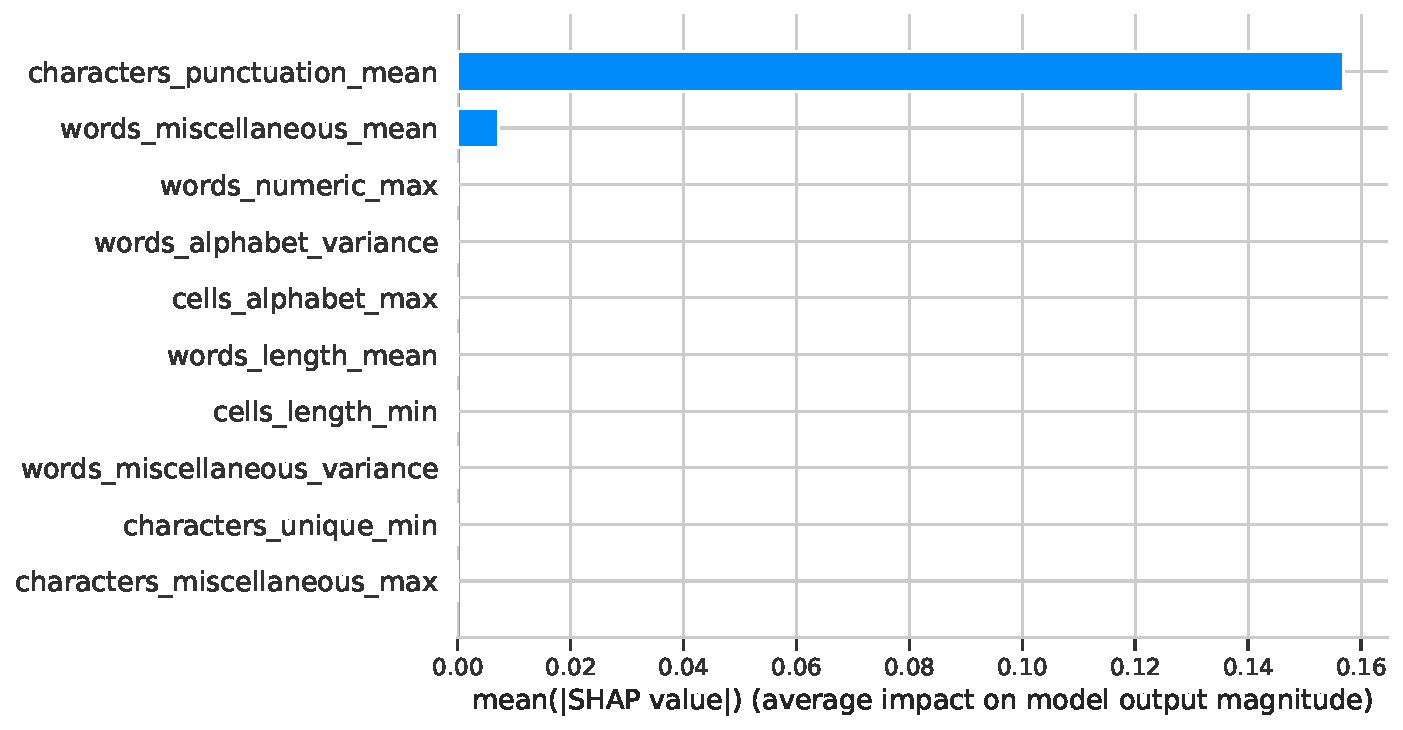
\includegraphics[width=0.9\textwidth]{thesis/Figures/RQ4/Shap_cell_rec_KATARA.pdf}
    \caption{KATARA - Top 10 Recall influential features according to SHAP values}
    \label{fig:feature_importance_rec_KATARA}
\end{figure}

\begin{table}[H]
	\centering
	\addtolength{\leftskip} {-2cm}
	\addtolength{\rightskip}{-2cm}
	\captionsetup[subtable]{position = below}
	\captionsetup[table]{position=top}
	\caption{Top feature influences - KATARA}
	\label{tab:feature_influences_KATARA}
		\begin{subtable}{0.5\linewidth}
		\centering
\begin{tabular}{llr}
\toprule
 \# &                         Feature &        Influence \\
\midrule
 1 &       words\_alphabet\_variance &  0.29 $\nearrow$ \\
 2 &         cells\_length\_variance &  -0.2 $\searrow$ \\
 3 &  characters\_alphabet\_variance &  0.11 $\nearrow$ \\
\bottomrule
\end{tabular}

		\caption{Precision feature influences - KATARA}
		\label{tab:prec_feature_influences_KATARA}
	\end{subtable}
	\hspace*{4em}
	\begin{subtable}{0.5\linewidth}
		\centering
\begin{tabular}{llr}
\toprule
 \# &                        Feature &            Influence \\
\midrule
 1 &  characters\_punctuation\_mean &  -0.05 $\rightarrow$ \\
 2 &     words\_miscellaneous\_mean &     -0.07 $\searrow$ \\
 3 &            words\_numeric\_max &      0.38 $\nearrow$ \\
\bottomrule
\end{tabular}
		\caption{Recall feature influences - KATARA}
		\label{tab:rec_feature_influences_KATARA}
	\end{subtable}%
\end{table}

% ---------------------------------------------
% ---------------------------------------------
% ---------------------------------------------
% ---------------------------------------------
% ---------------------------------------------
% ---------------------------------------------


\subsubsection{Raha}
\begin{figure}[H]
    \centering
    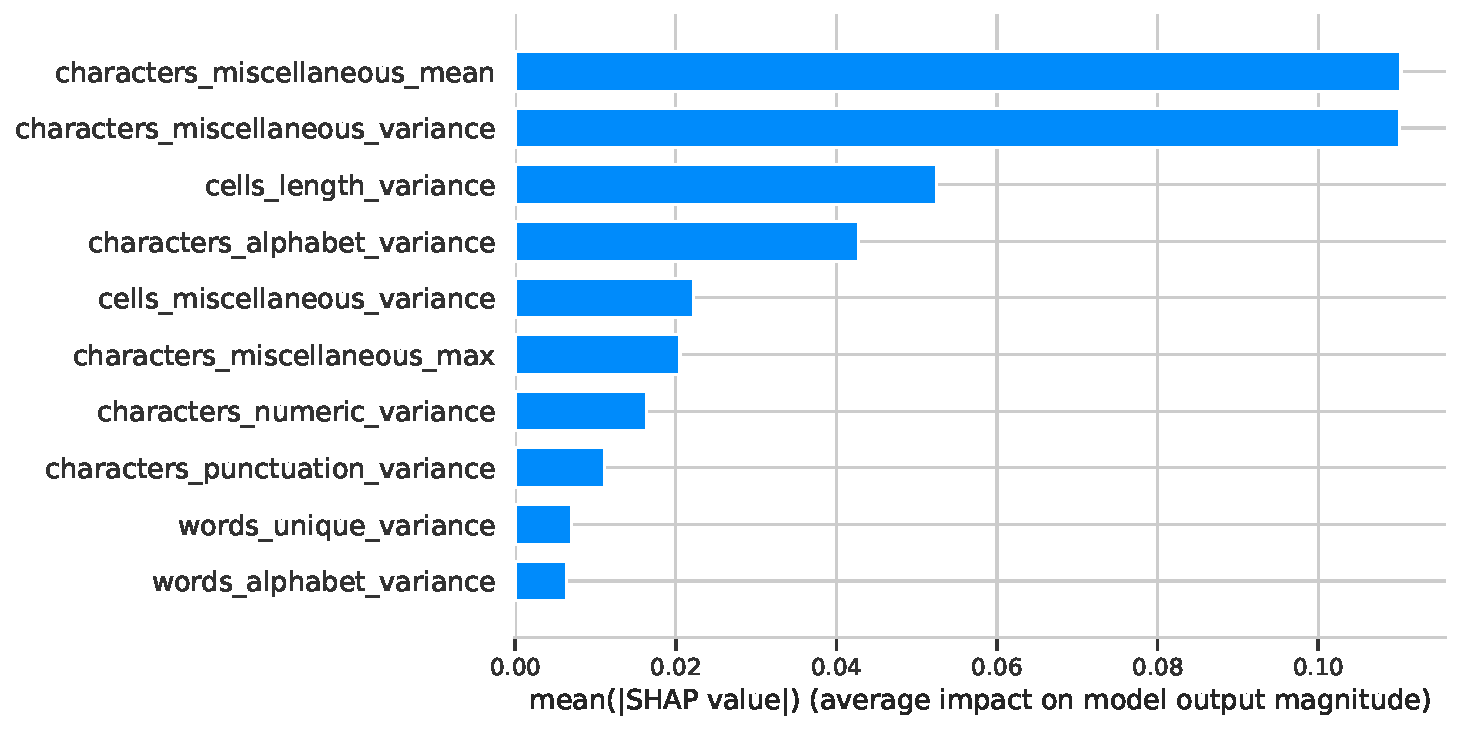
\includegraphics[width=0.9\textwidth]{thesis/Figures/RQ4/Shap_cell_prec_Raha.pdf}
    \caption{Raha - Top 10 Precision influential features according to SHAP values}
    \label{fig:feature_importance_prec_Raha}
\end{figure}
\begin{figure}[H]
    \centering
    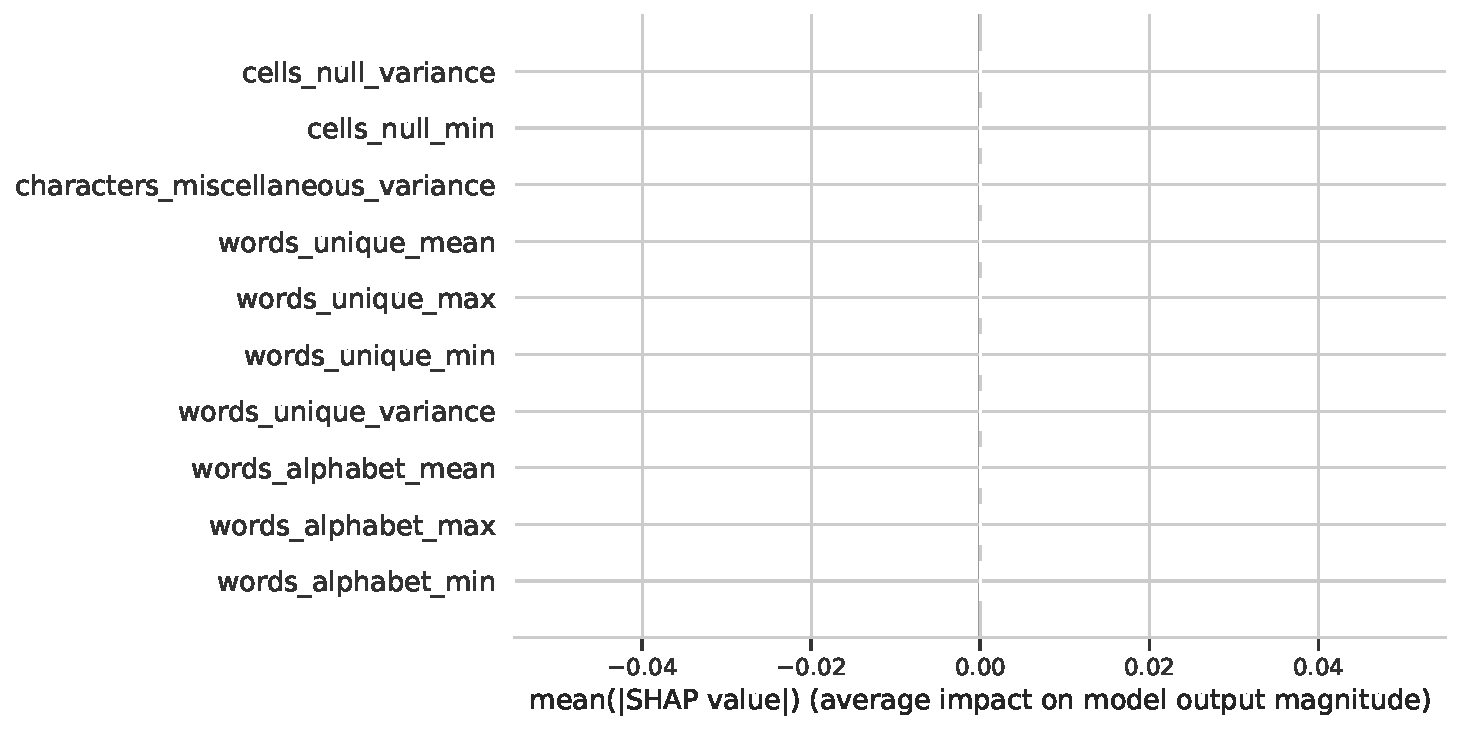
\includegraphics[width=0.9\textwidth]{thesis/Figures/RQ4/Shap_cell_rec_Raha.pdf}
    \caption{Raha - Top 10 Recall influential features according to SHAP values}
    \label{fig:feature_importance_rec_Raha}
\end{figure}

\begin{table}[H]
	\centering
	\addtolength{\leftskip} {-2cm}
	\addtolength{\rightskip}{-2cm}
	\captionsetup[subtable]{position = below}
	\captionsetup[table]{position=top}
	\caption{Top feature influences - Raha}
	\label{tab:feature_influences_Raha}
		\begin{subtable}{0.5\linewidth}
		\centering
		\begin{tabular}{llr}
\toprule
 \# &                              Feature &         Influence \\
\midrule
 1 &      characters\_miscellaneous\_mean &  -0.42 $\searrow$ \\
 2 &  characters\_miscellaneous\_variance &  -0.35 $\searrow$ \\
 3 &              cells\_length\_variance &   -0.2 $\searrow$ \\
\bottomrule
\end{tabular}
		\caption{Precision feature influences - Raha}
		\label{tab:prec_feature_influences_Raha}
	\end{subtable}
	\hspace*{4em}
	\begin{subtable}{0.5\linewidth}
		\centering
\begin{tabular}{llr}
\toprule
 \# &                              Feature & Influence \\
\midrule
 1 &                cells\_null\_variance &         0 \\
 2 &                     cells\_null\_min &         0 \\
 3 &  characters\_miscellaneous\_variance &         0 \\
\bottomrule
\end{tabular}
		\caption{Recall feature influences - Raha}
		\label{tab:rec_feature_influences_Raha}
	\end{subtable}%
\end{table}

\newpage
\subsection{Evaluation}
\newpage
